\documentclass[12pt, letterpaper]{scrartcl}

\usepackage{fullpage} % Set margins and place page numbers at bottom center
\usepackage[shortlabels]{enumitem} % Use a. in the enumerate
\usepackage{amsmath} % aligned equations
\usepackage{graphicx} % include figure
\usepackage{float} % usage of H for figure float
\usepackage{amssymb} % \blacksqure and \triangleq
\usepackage{xcolor} % color in math mode

\begin{document}

% ### Header - start ###
    \begin{center}
    	\hrule
    	\vspace{0.4cm}
    	{\textbf { {\large Homework 3} \\ EE 668 --- Information Theory}}
    \end{center}
    { \textbf{Name:} Ali Zafari \hspace{\fill} \textbf{Student Number:} 800350381 \hspace{\fill} \textbf{Fall 2022} } \newline\hrule
% ### Header - end ###

\paragraph*{Problem 3.1} \hfill\newline
\begin{enumerate}[((a))]
    \item
    Graph below shows binary Hufffman codes.
    \begin{figure}[H]
        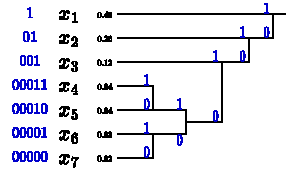
\includegraphics[width=0.5\linewidth]{hw3_figures/3.1a.pdf}
        \centering
    \end{figure}
    
    \item 
    The average codeword length is:
    \begin{align*}
        L_{avg} = 0.49\times1+0.26\times2+0.12\times3+0.04\times5+0.04\times5+0.03\times5+0.02\times5=2.02 \quad[bits]
        %0.49*1+0.26*2+0.12*3+0.04*5+0.04*5+0.03*5+0.02*5
    \end{align*}
    
    \item
    Graph below shows ternary Hufffman codes.
    \begin{figure}[H]
        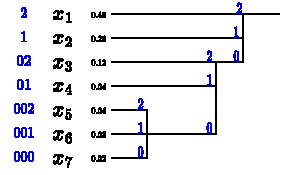
\includegraphics[width=0.5\linewidth]{hw3_figures/3.1c.pdf}
        \centering
    \end{figure}
\end{enumerate}
\hrule

\paragraph*{Problem 3.2} \hfill\newline
\begin{enumerate}[((a))]
    \item
    Huffman code with code lengths $(1,2,3,3)$:
    \begin{figure}[H]
        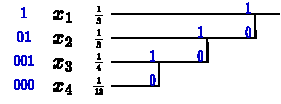
\includegraphics[width=0.5\linewidth]{hw3_figures/3.2a.pdf}
        \centering
    \end{figure}
    
    \item
    Huffman code with code lengths $(2,2,2,2)$:
    \begin{figure}[H]
        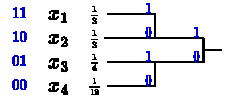
\includegraphics[width=0.5\linewidth]{hw3_figures/3.2b.pdf}
        \centering
    \end{figure}
    
    \item
    Shannon code lengths are listed below. As can be seen in part (a), there are 2 codes with length 3, which is higher than length of two, as Shannon code offered.
    \begin{center}
        \begin{tabular}{ c c c} 
         \hline
         \\$x$ & $P(x)$ & $l_{Shannon}(x)=\lceil\log{\frac{1}{p(x)}}\rceil$\\\\
         \hline
         $1$ & $1/3$ & $2$\\
         $2$ & $1/3$ & $2$  \\
         $3$ & $1/4$ & $2$ \\
         $4$ & $1/12$ & $4$  \\
         \hline
        \end{tabular}
    \end{center}
\end{enumerate}
\hrule

\paragraph*{Problem 3.3} \hfill\newline
\begin{enumerate}[((a))]
    \item
    \begin{align*}
        H(p)=-\sum p(x)\log p(x)=1.875
    \end{align*}
    \begin{align*}
        H(q)=-\sum q(x)\log q(x)=2
    \end{align*}
    \begin{align*}
        D(p||q)=\sum p(x)\log \frac{p(x)}{q(x)}=0.125
    \end{align*}
    \begin{align*}
        D(q||p)=\sum q(x)\log \frac{q(x)}{p(x)}=0.125
    \end{align*}
    \item
    \begin{align*}
        L_{{C_1}_{avg}}=\sum p(x)l_{C_1}(x)=1.875=H(p)
    \end{align*}
    \begin{align*}
        L_{{C_2}_{avg}}=\sum q(x)l_{C_2}(x)=2=H(q)
    \end{align*}
    \item
    \begin{align*}
        L_{{C_2}_{avg}}=\sum p(x)l_{C_2}(x)=2
    \end{align*}
    The average length differs by amount of $D(p||q)$ from the actual entropy $H(p)$.
    \item 
    \begin{align*}
        L_{{C_1}_{avg}}=\sum q(x)l_{C_1}(x)=2.125
    \end{align*}
    The average length differs by amount of $D(q||p)$ from the actual entropy $H(q)$.
\end{enumerate}
\hrule

\paragraph*{Problem 3.4} \hfill\newline
\begin{center}
    \begin{tabular}{ c c c c c c c } 
     \hline
     \\$x$ & $P(x)$ & $F(x)$ & $\overline{F(x)}$ &$\overline{F(x)}$ in Binary & $l(x)=\lceil\log{\frac{1}{p(x)}}\rceil+1$ & Codeword\\\\
     \hline
     $1$ & $0.04$ & $0.04$ & $0.02$ & $0.000001010001111011$ & $6$ & $000001$ \\
     $2$ & $0.08$ & $0.12$ & $0.08$ & $0.0001010001111010111$ & $5$ & $00010$ \\
     $3$ & $0.16$ & $0.28$ & $0.20$ & $0.00110011001100110011$ & $4$ & $0011$ \\
     $4$ & $0.20$ & $0.48$ & $0.38$ & $0.01100001010001111011$ & $4$ & $0110$ \\
     $5$ & $0.24$ & $0.72$ & $0.60$ & $0.1001100110011001101$ & $4$ & $1001$ \\
     $6$ & $0.28$ & $1.00$ & $0.86$ & $0.11011100001010001111$ & $3$ & $110$ \\
     \hline
    \end{tabular}
\end{center}


The average codeword length is:
\begin{align*}
    L_{avg} = 0.04\times6+0.08\times5+0.16\times4+0.20\times4+0.24\times4+0.28\times3=3.88 \quad[bits]
    %0.04*6+0.08*5+0.16*4+0.20*4+0.24*4+0.28*3
\end{align*}

Entropy of the random variable:
\begin{align*}
    H(X) = 2.37
    %0.04*log2(0.04)+0.08*log2(0.08)+0.16*log2(0.16)+0.20*log2(0.20)+0.24*log2(0.24)+0.28*log2(0.28)
\end{align*}

\emph{Shannon-Fano-Elias} coding guarantees an average codelength of less than $H(X)+2$ which is satisfied here.\\
\hrule

\paragraph*{Problem 3.5} \hfill\newline
\begin{align*}
    \frac{\partial}{\partial d_1}J(d_1,d_2)+\lambda\frac{\partial}{\partial d_1}(d_1+d_2-D) + \mu_1\frac{\partial}{\partial d_1}(d_1-\sigma_1^2)=0\\
    \frac{\partial}{\partial d_2}J(d_1,d_2)+\lambda\frac{\partial}{\partial d_2}(d_1+d_2-D) + \mu_2\frac{\partial}{\partial d_2}(d_2-\sigma_2^2)=0
\end{align*}
We now consider first that inequality conditions are satisfied ($\mu_i=0$)
\begin{align*}
    -\frac{1}{d_1}+\lambda+0=0 \longrightarrow d_1 = \frac{1}{\lambda}\\
    -\frac{1}{d_2}+\lambda+0=0 \longrightarrow  d_2 = \frac{1}{\lambda}
\end{align*}
If we consider $\mu_i<0$:
\begin{align*}
    -\frac{1}{d_1}+\lambda+\mu_1=0 \longrightarrow \mu_1<0\longrightarrow d_1 < \frac{1}{\lambda}\\
    -\frac{1}{d_2}+\lambda+\mu_2=0 \longrightarrow \mu_2<0\longrightarrow d_2 < \frac{1}{\lambda}
\end{align*}
To find the value of $\lambda$ we use the equality constraint:
\begin{align*}
    d_1+d_2=D \longrightarrow \frac{2}{\lambda}=D \longrightarrow \lambda=\frac{D}{2}
\end{align*}
Therefore, dividing the total distortion ($D$) evenely on both channels, would give us the minimum loss trade-off in rate-distortion measurement. ($(d_1,d_2)=(\frac{D}{2}, \frac{D}{2})$)\\
\hrule

\paragraph*{Problem 3.6} \hfill\newline
\begin{align*}
    f(x,y)=14x-x^2+6y-y^2+7
\end{align*}
Constraints:
\begin{align*}
    x+y&\leq 2\\
    x+y&\leq \frac{3}{2}
\end{align*}
First check for local maxima:
\begin{align*}
    \frac{\partial}{\partial x}f(x,y)=14-2x=0 \longrightarrow x=7
\end{align*}
\begin{align*}
    \frac{\partial}{\partial y}f(x,y)=6-2y=0 \longrightarrow y=3
\end{align*}
point $(7, 3)$ is out of the constraints, therefore it is not a solution.\\
Checking the boundaries: (the second boundary already satisfies the first one, so we only check the second one)
\begin{align*}
    x+y=\frac{3}{2}
\end{align*}
\begin{align*}
14-2x=\lambda \longrightarrow x = \frac{14-\lambda}{2}\\
6-2y=\lambda \longrightarrow y = \frac{6-\lambda}{2}
\end{align*}
Then we solve for the Lagrangian over the boundary:
\begin{align*}
\frac{14-\lambda}{2}+\frac{6-\lambda}{2}=\frac{3}{2} \longrightarrow \lambda=\frac{17}{2} 
\end{align*}
So the possible solution will be: $(\frac{11}{4}, \frac{-5}{4})$ which is on the boundary, so it is the final solution to the constrained optimization.
(If both contraints assumed active, the system of equations will have no solution)\\
Finally, the maximum value of $f(x,y)$ in this constrained domain will be:
\begin{align*}
    f(\frac{11}{4}, \frac{-5}{4})=28.875
\end{align*}
\hrule

\end{document}

